% copyright (c) 2015 Synrc Research Center

\documentclass[11pt,oneside]{article}
% Copyright (c) 2010 Synrc Research Center

\usepackage{ifthen}
\usepackage[english,russian]{babel}
%\usepackage{palatino}
\usepackage{graphicx}
\usepackage{cite}
\usepackage{hyperref}
\usepackage[utf8]{inputenc}
\usepackage{moreverb}
\usepackage{listings}
%\usepackage{hevea}
\usepackage[none]{hyphenat}
\usepackage{caption}
\usepackage[usenames,dvipsnames]{color}
\usepackage[hmarginratio=2:3]{geometry}

\hyphenation{framework nitrogen javascript facebook}

% include image for HeVeA and LaTeX

\makeatletter
\def\@seccntformat#1{\llap{\csname the#1\endcsname\quad}}
\makeatother

\newcommand{\includeimage}[2]
{\ifhevea
    {\imgsrc{#1}}
\else{
    \begin{figure}[h!]
    \centering
    \includegraphics[width=\textwidth]{#1}
    \caption{#2}
    \end{figure}}
\fi}

\lstset{
    backgroundcolor=\color{white},
    keywordstyle=\color{blue},
    basicstyle=\bf\ttfamily\footnotesize,
    columns=fixed}

\headsep = 0cm
\voffset = 0cm
\hoffset = 1cm
\topmargin = 0cm
\textwidth = 15cm
\textheight = 22cm
\footskip = 1.3cm
\parindent = 0cm

\hyphenpenalty=5000
  \tolerance=1000

\newcommand{\sign}[1]{%      
  \begin{tabular}[t]{@{}l@{}}
  \makebox[1.5in]{\dotfill}\\
  \strut#1\strut
  \end{tabular}%
}
\newcommand{\Date}{%
  \begin{tabular}[t]{@{}p{1.5in}@{}}
  \\[-1ex]
  \strut Date: \dotfill\strut
  \end{tabular}%
}

\begin{document}

\thispagestyle{empty}
\begin{center}

\begin{minipage}[t]{2cm}
    
\includegraphics[scale=0.4]{img/S}
\end{minipage}
\begin{minipage}[t]{12cm}
    \begin{flushright}
        \textsc{{\Large {\bf {\color{Blue}syn}{\color{OrangeRed}rc} research center s.r.o.}}}\\
        \textsc{Roháčova 141/18, Praha 3 13000, Czech Republic}\\
    \end{flushright}
\end{minipage}

\vspace{3cm}

    \vspace{3cm}   {\Large \bf Системна інженерія та верифікація\\ \vspace{0.2cm} уніфікованого обчислювального середовища}\par
    \vspace{1cm}   {\Large \bf System Engineering and Verification\\ \vspace{0.2cm} of Unikernel Execution Environment}\par
    \vspace{3cm}   {\Large Павло Маслянко, Київський Політехнічний Інститут\par}
    \vspace{0.3cm} {\Large Максим Сохацький, Synrc Research Center\par}
    \vspace{4cm}   {\Large Листопад 2015}

\end{center}

\vspace{2cm}
\newpage
\section{Вступ}

\vspace{1cm}

%\vspace{0.5cm}

\subsection{Системна інженерія}

   Протягом історії обчислювальної техніки було створено різні класи та способи обчислень,
   різні тоеорії та підходи до програмування таких систем, різні класи систем програмування.
   Зараз уже стало зрозумілим, що інженіринг систем які не піддаються до верифікації
   формальними методами не може бути застосований у галузях де вимоги до якості
   особливо підвищені, як то космонавтика, енергетика та телекомунікації.

\subsection{Уніфіковані обчислювальні середовища}

   Називатимемо програмні комплекси та системи, які розповсюджуються на всі прошарки моделі OSI вище фізичного,
   уніфікованими середовищами. Перелічуючи проекти, які вплинули на хід історії
   обчислювальної техніки, серед такого уніфікованих замкнених систем, можна згадати Smalltalk-80,
   створений в Xerox Parc Аланом Кеєм, якого можна назвати творцем об'єктно-орієнтованого підходу, за що він був
   удостоєний премії Тюрінга. Віртуальні машини середовища Smalltalk представляють відносно ізольовано
   по відношенню до операційної системи систему типів разом з моделью акторів, що дозволяє
   самостійно розподіляти час обчислювального середевища. Стан таких віртуальних апаратно незалежний
   та може бути перенесений на віртуальні машини які працюють на процесорах інших архітектур.
   Інший класс систем які були представлені у той час -- це Lisp машини. Вони теж були
   здатні зберігати стан своєї віртуальної машини яка,
   як і усе середовище була написана на мові Lisp. Серед експериментальних та науково-дослідних
   уніфікованих систем можна відзначити Singularity від Microsoft Research, яка давно є постачальником
   високоякісних теоретико-практичних інструментів по веріфікації програмного забезпечення.
   Сучасні унфіковані системи існують на трьох мовах програмування (на OCaml це MirageOS,
   на Haskell це HaLVM, для Erlang це віртуальна машина LING, яка створена в Україні) та
   здатні виконуватися без операційної системи. В даній роботі дається обгрунтуванню вибору
   віртуальної машини Erlang та її операційної семантки у якості основи для обчислювального
   середовища та його сервісів.

   \paragraph{}
   Застосовуючи формальні методи доведення коректності велику частину має повнота за макненість системи,
   адже недоведені або неверифіковані частини можуть вплинути на детермінованість а отже якість системи.
   Тому має велике значення забезпечення виконання системи якогомога ближче до аппаратного забезпечення.
   Основні напрямки побудови замкнених середовищ на функціональних мовах програмування існують для мов Erlang, Haskell та OCaml.

\newpage
\subsection{Верифікація}

   \paragraph{}
   За багато років кількість теорій, які використовуються для побудови програмного забезпечення значно розширилися:
   починаючи з теорії компіляції сучаних функціональних мов, та систем програмування на основі теорії типів,
   включаючи сучасні моделі обчислень, які побудовані на основі лямбда числення та числення процесів, закінчуючи віртуальними
   машинами які працююсь у семантиці захищених, простих за структурою процесів, час яких розподіляється
   у прозорий та ефективний спосіб.

   \paragraph{}
   Розглядаючи системи, які піддаються формальній верифікації, кажуть про
   сертифіковане або верифіковане програмне забезпечення. Серед логічних систем, які
   застосовувалися для цього можна відзначити клас темпоральних логік для доведення
   цілісності разподілених у просторі та часі систем (приклали таких систем: NuPRL від університету Корнела в Нью-Йорку;
   TLA+ фреймворк Леслі Лампорта за який він отримав премію Тюрінга від Microsoft Research), а також системи з залежними
   типами (теорія типів Мартіна Льофа) побудовані на основі числення індуктивних конструкцій (приклади таких систем:
   Coq побудована на мові OCaml від національного науково-дослідного інституту Франції INRIA;
   Agda побудовані на мові Haskell від швецького інституту технологій Чалмерс;
   Lean побудована на мові C++ від Microsoft Research та Універсистету Каргені-Мелона).

\subsection{Компактні протоколи}

   Зараз на планеті налічується близько 50 міліардів пристроїв які повинні обслуговуватися
   масштабованими ефективними серверними комплексами які гарантовано не виконують
   додаткових та непотрібних обчислень. Це потребує повного перепроектування усіх протоколів
   які виникають між компонентнами та підсистемами. Ця работа також представляє
   уніфікований та простий стек протоколів розроблюваного обчислювального середовища.

   \begin{center}
   \vspace{0.5cm}
   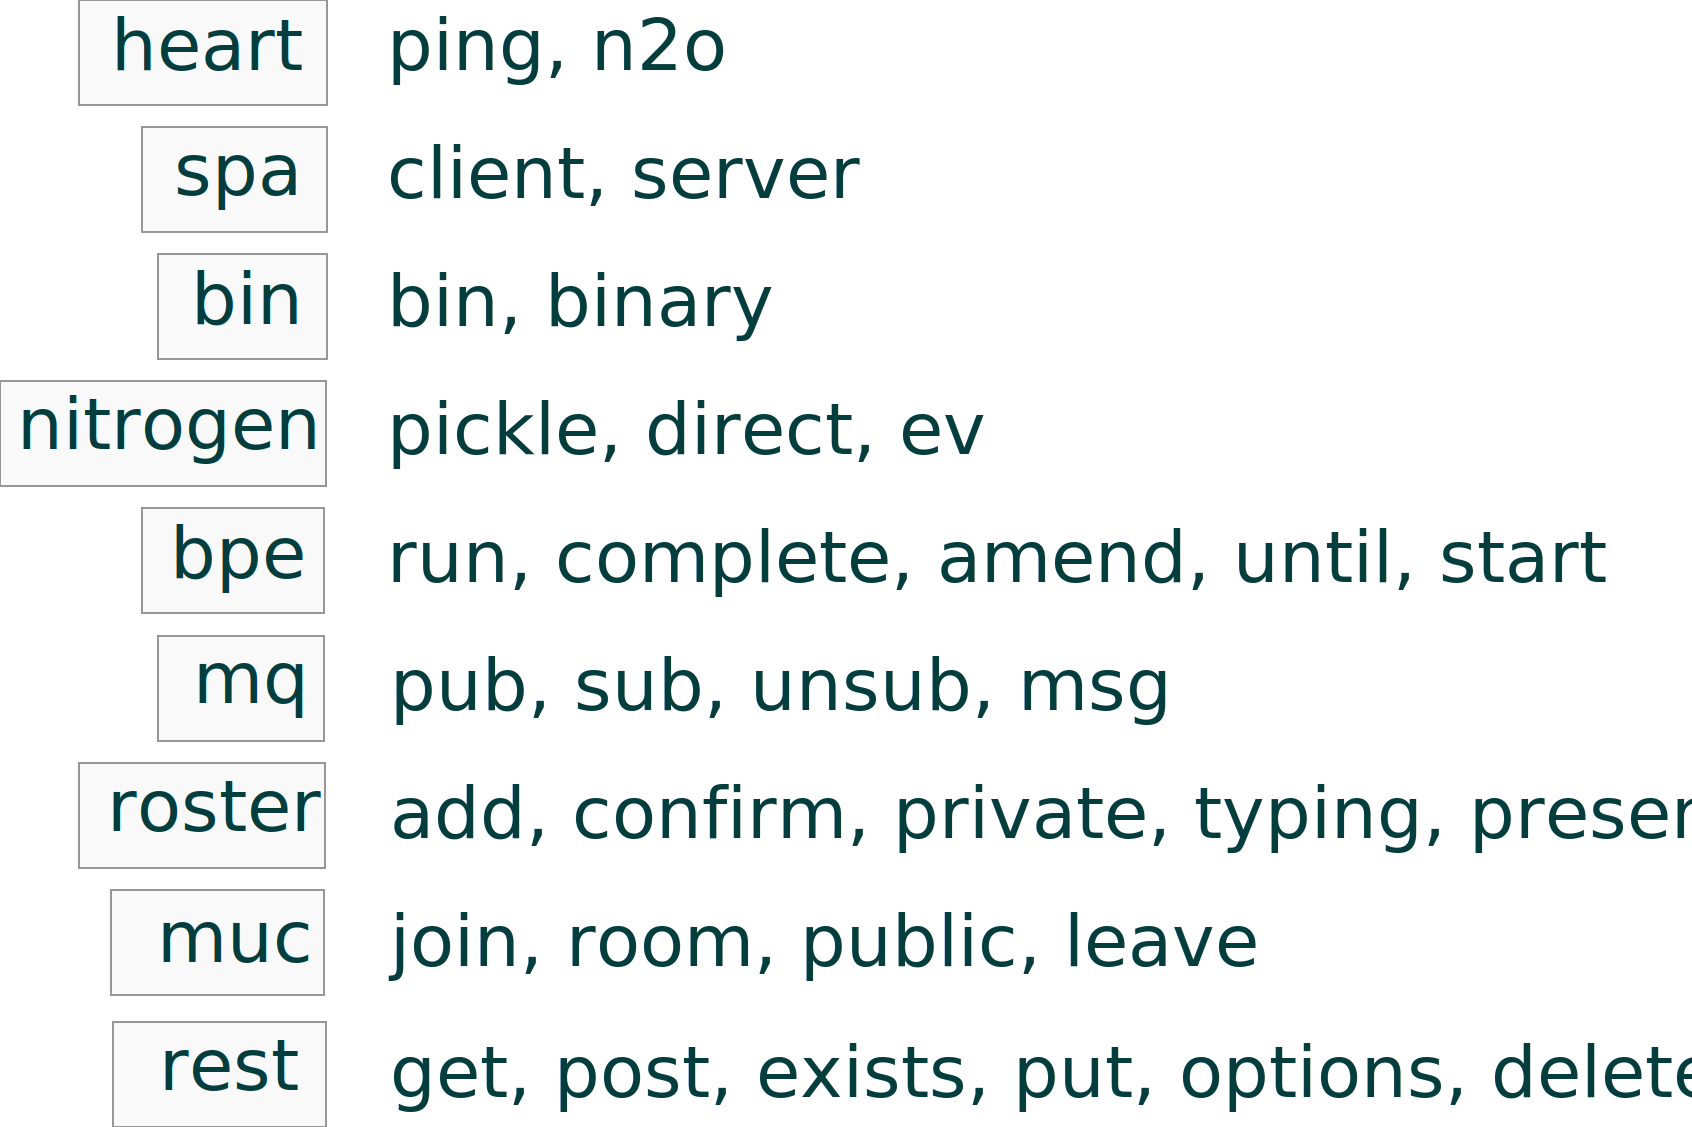
\includegraphics[scale=0.15]{img/protocols}
   \end{center}

\newpage

\subsection{Завдання дослідження}

   Тактична мета даної роботи -- це реалізація усіх верхніх компонентів OSI на базі
   формальної теорії та мови з залежнити типами. Побудова зручної сучасної гнучкої верифікованої теорії
   з компактною системою типів є основним завданням даної роботи. Будемо орієнтуватися
   на мінімально можливу систему типів та набір функцій які забезпечать успішне промислове
   впровадження кінцевого продукту.

   \paragraph{}
   Таким чином будемо орієнтуватися на практичне застосування прикладних сервісів,
   з компактною та достатньо потужною системо типів. В першу чергу мова йде про три найголовніші
   сервіси: збереження інформації, система управління процесами та мультиплікатор протоколів,
   який у даній системі відіграє роль сервера додатків. Успішна реалізація цих трьох систем
   дасть нам змогу будувати більш складні та масштабовані транзакційні системи та сервіси на базі
   створеної формальної теорії, а також прокладе шлях подальшому розвитку даного
   теоретико-практичного комплексу.

   \begin{center}
   \vspace{0.5cm}
   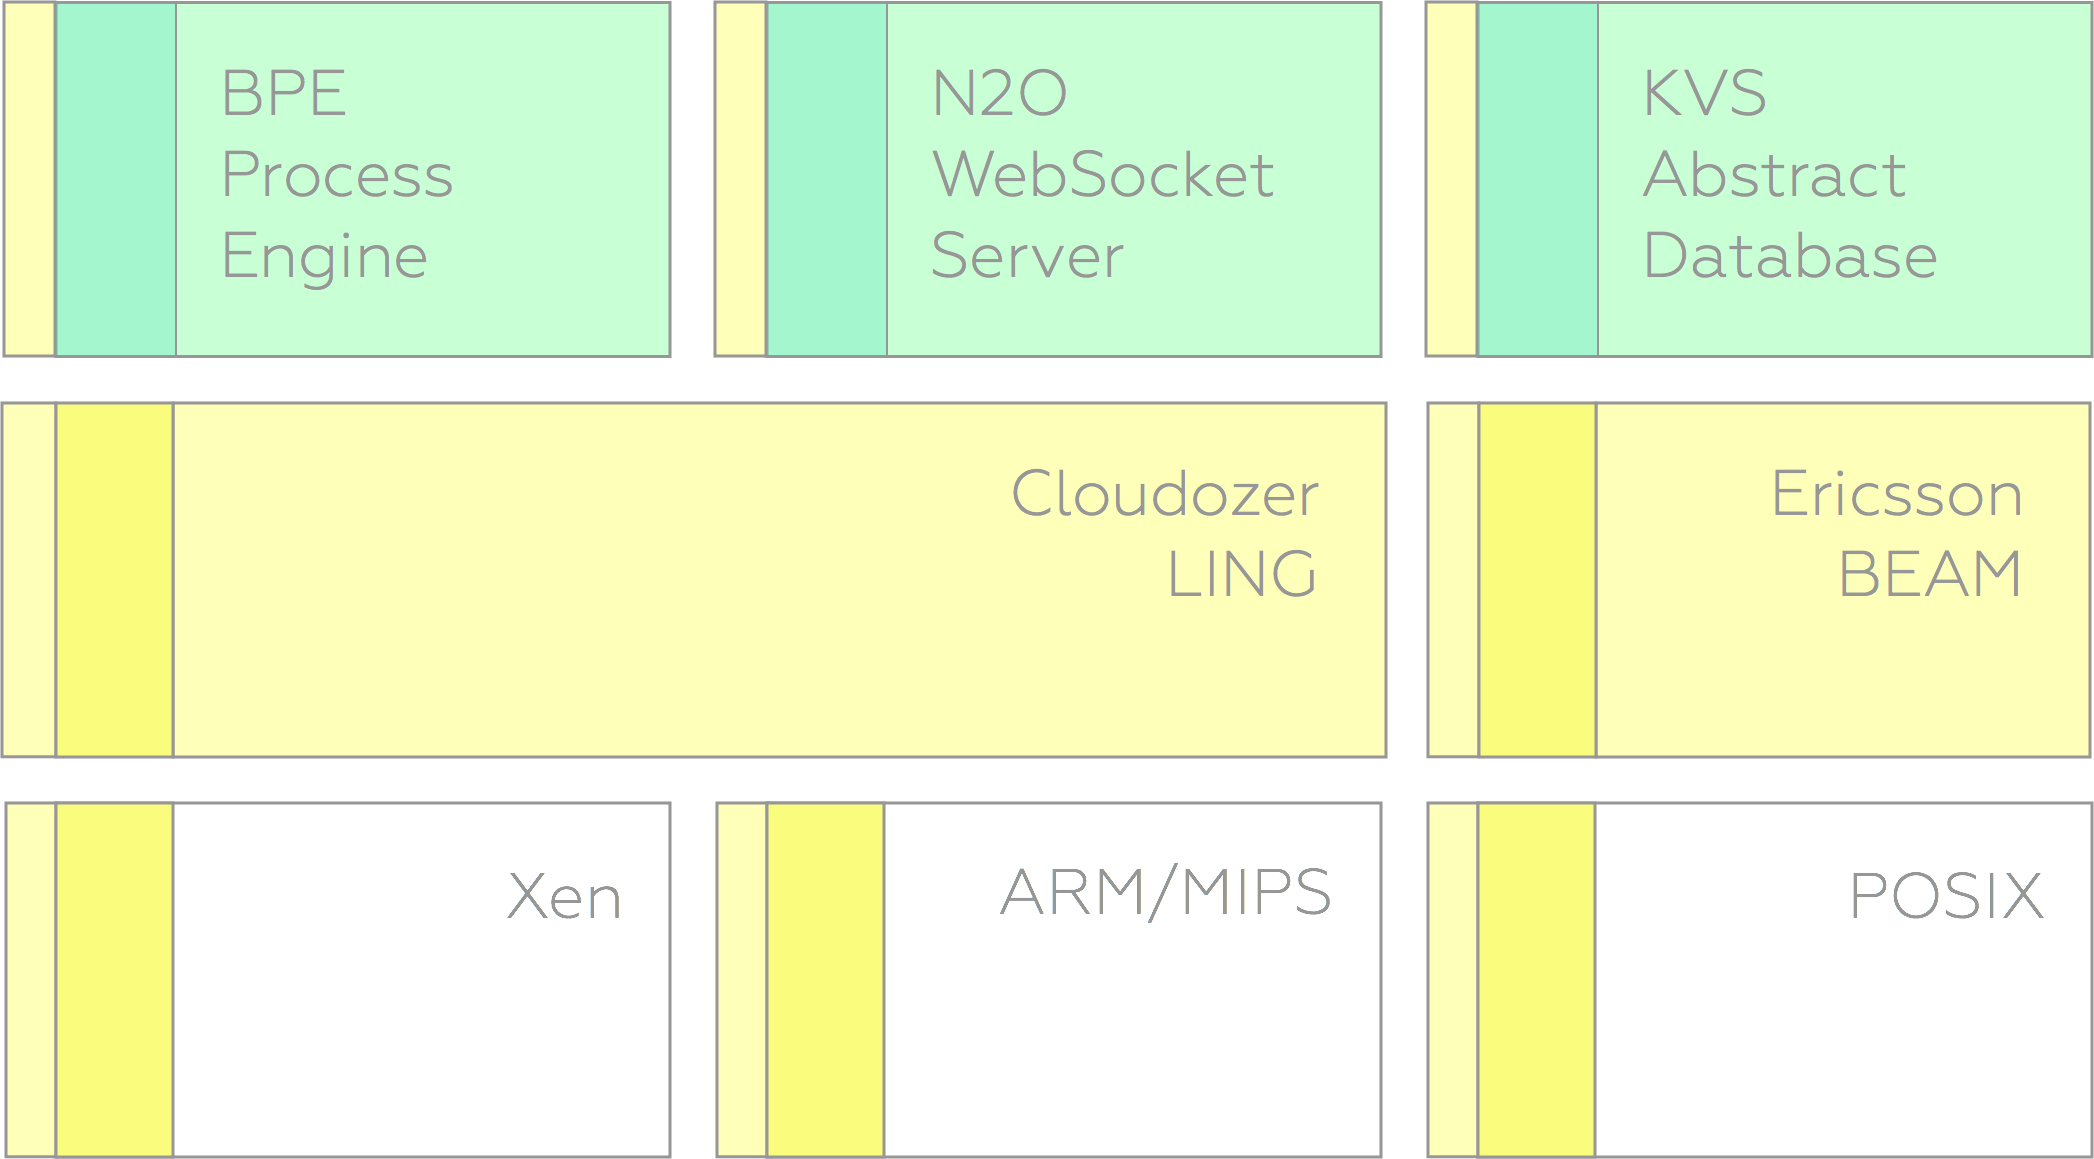
\includegraphics[scale=0.15]{img/exe-res}
   \end{center}

   \paragraph{}
   Що стосується апаратної частини моделі OSI, то тут ми будемо вважати умовно,
   що аппаратне забезпечення і так проходить усі належні види моделювань, такі як
   розрахункові імітаційні та інші. Крім того як ми знаємо верифіковані моделі уже застосовуються
   для розробки мікропроцесорів.

   \paragraph{}
   Верифікована система типів середнього рівня моделі OSI --- віртуальної машини
   є предметом майбутніх досліджень. Адам Чіпала \cite{chipvm} показав як можно
   верифікувати виконання команд віртуальної машини та компіляцію цих команд в байт-код.

   \paragraph{}
   Верифікована система типів верхнього рівня моделі OSI --- це центральний фокус даногої роботи.
   Ми розглянемо декільки основних сервісів які стосуються безпосередньо управління даними та їх стрктурами,
   та сервісів управління обчисленнями.

   \newpage

\subsection*{Зберігання обчислень}
   \paragraph{}
   У цій роботі ми будемо верифікувати системні бібліотеки для
   майбутньої верифікованої віртуальної машини. Зокрема значна увага буде приділятися
   послідовностям. Система персистентного зберігання послідовностей є ядром нашого
   обчислювального середовища. Властивості цієї підсистеми є основоположними
   для перевірки констистентності операційних логів розподілених базах данних.


\subsection*{Виконання процесів}
   \paragraph{}
   Тут ми дамо формальне визначення та верифікуємо
   типи системи управління структурованими процесами або FSM автоматами.
   Бізнес-процеси це зручний та ефективний спосіб упорядкування та формалізації
   потоків даних. Ми зосередимося на найкомактніших алгебрах.

\subsection*{Комутація протоколів}
   \paragraph{}
   Ця частина дасть відповіть на питання структуровання
   протоколів та визначення універсального мультиплікатора. Буде описаний повний стек
   протоколів для IoT та WebSocket додатків.

\subsection*{Розподілені у просторі та часі системи}

   \paragraph{}
   Сучасний розвиток техніки та теоретична межа швидкості обробки процесорів вивів на передній план алгоритми та структури
   данних які ефективно використоують розподілені у просторі та часі ресурси, як то об’єми памяті та обчислювальні потужності.
   Принципи та підходи паралельного та узгодженого програмування дають змогу масштабувати системи та обчисленя, однак
   анонсують нові теорії для забезпечення коректності в умавах підвищеної складності алгоритмів у розподілених системах,
   такі як алгоритми забезпечення консистентності та транзакційності у розподілених системах PAXOS та CR.
   Сучасні обчислювальні середовища повинні ефективно управляти великими масивами
   даних та необмежено масштабуватися. Розподілена архтітектура сервера транзакцій
   які працюють поверх формального верифікованого сховища даних буде представлена
   окремою роботою. Даний прототип існує у вигляді координатора транзакцій який працью
   за алгоритмом ланцюгової реплікації і використовує семантику сховища, яке
   у формальному вигляді представлене у цій роботі.

\subsection*{Дотичні формальні теорії}

   Важливо додати, що з формальної точки зору потрібно щоби на границях
   трьох системних рівнів формальні типи дотичних логічних теорій співпадали.
   Для доведення коректності формалізовної віртуальної машини достатньо
   визначити систему типів команд мови процессор та типи їх операндів. А для
   доведення коректності верхнього рівня достатньо аксіоматизувати дотичну
   формальну теорію віртуальної машини. Тому в даній роботі буде представлена
   така публічна система типів віртуальної машини що одразу відкриє дорогу
   для деталізації і подальшої теоретичної розробки формальної теорії для віртуальної машини.

\newpage

\subsection{Структура роботи}

   \paragraph{}
   Покладаючись на аналіз рішень в області уніфікованих середовищ та
   набір математичного і лінгвістистичного забезпечення у якості формальних методів,
   ми будемо формувати формальну теорію та бібліотеку типів для формальної
   реалізації ключових підсистем.

   \paragraph{}
   Усі існуючі уніфіковоані системи, оскільки є замкеними, пропонують
   повністю свій інтерфейс взаємодії, свою операціїну семантку та свою систему типів.
   У цьому смислі наша система не є винятком і пропонує повний стек
   програмного забезпечення, ключові частини якого ми намагатимемося формально
   описати.

   \paragraph{}
   На основі створеної базової теорії та її бібліотеки типів ми створимо
   формальними методами доказову базу для кожного компонена обчислювального
   середовища, який включений в дану роботу: {\bf зберігання обчислень},
   {\bf виконання процесів}, {\bf мультиплікатор протоколів}.

   \paragraph{}
   Далі кожна така верифікована система буде транслюватися в цільову мову
   віртуальної машини обчислювального середовища, яка у загальному випадку
   може відрізнятися від вибраної нами Erlang.

   \paragraph{}
   Особливість цієї уніфікованої системи в повному та тотальному перегляді
   усіх існуючих рішень включно з базовими протоколами інтернету типу HTTP.
   Так наприклад для сервера додатків у якості транспортного протоколу
   використовується бінарний WebSocket протокол. Усі протоколи формулюються
   у вигляді алгебр над станами процесів.

\subsection*{Уніфіковані обчислювальні середовища}

   \paragraph{}
   Об’єктом дослідження є усі можливі моделі обчислювальних середовищ в основному придатних
   до верифікованого аналізу та обробки формальними методами. Ми вибрали середовище
   основані на віртуальних машинах зі своєю системою типів та байткодом, які уже
   використовуюються у промисловій експлуатації в телекомунікайній сфері та є лідерами
   у цій області це телекомукаційна платформа Ericsson -- Erlang/OTP. Ступінь проникнення
   цієї технологій у сучасних телекомунікаціях достатньо високий, особливо завдяки
   розвиненій підтримці ASN.1, SNMP, H.262, Radius та інших промислових стандартів
   у телекомунікаційній сфері. Перші успішні масштабні проекти на Erlang були створені ще у
   1986 році, а зараз Erlang демонструє успішність завдяки таким проектам як WhatsApp, який
   обслуговує 30 міліардів повідомлень в день у порівнянні з SMS трафіком,
   який генерується щоденно у розмірі 20 міліардів повідомлень.

\newpage

\subsection*{Формальні методи}

   \paragraph{}
   Самі формальні методи теж є частиною об’єкта дослідження. Ми досліджуємо ті структури
   та алгоритми які дадуть максимально ефективний спосіб кодування та виконнання,
   забезпечуючи при цьому семантику, яка використовуються для машинного доведення
   коректності роботи алгоритмів та узгодженості міжпроцесних протоколів.
   Ми будемо розробляти робочу формальну теорію за допомогою індуктивних типів,
   переводячи результати на мову обчислювального середовища, Erlang.

   \paragraph{}
   Побудова розподілених та паралельних, тобто здатних виконуватися на багатьох машинах одночасно, та
   узгоджених, тобто не блокуючих, а значить лінеаризованих систем управліннями процессами є побічним
   результатом який очікується від цієї роботи. Усі розподілені у просторі та часі
   протоколи ми будемо верифікувати використовуючи темпоральну логіку за допомогою системи TLA+.

\subsection*{Робоча теорія}

   \paragraph{}
   Вибравши конкретну систему автоматичного доведення теорем на основі теорії індуктивних типів,
   ми будуємо основні типи нашої теорії і визначаємо у нашій теорії сигнатури категорій підсистем
   нашого обчислювального середовища. Досліджуємо побудовану систему типів на предмет
   відповідності до робочого прототипу та доводимо певні властівості кожної із трьох
   підсистем включених до даної роботи.

\subsection*{Формальна підсистема}

   \paragraph{}
   Кожну окрему підсистему ми будемо відокремлювати та визначати які теореми
   та які констукції використовуються для побудови підсистеми формальним способом,
   використовуючи математичні конструкції робочої теорії. Розроблені теореми та сигнатури
   формальної підсистеми потім компілюються або транслюються в результуючу мову віртуальної машини
   обчислювального середовища. В нашому випадку це мова Erlang та віртуальні
   машини BEAM від Ericsson, та LING від Cloudozer. Для цього нам в базовії теорії доведеться
   формально описани базові примітиви віртуальної машини Erlang та взяти їх
   у якості аксіом для нашої теорії.

\subsection*{Результуюча підсистема}

\newpage
\subsection{Теоретичні сутності}
\vspace{0.5cm}
   У таксономії теоритичних сутностей умовно визначатимемо
   графічні топологічно- структурні, аналітичні, статистичні та логічні типи теорій, які
   ми використовуватимемо для опису комплесної теорії верифікованих середовищ
   послідовних обчислень розподілених узгоджених паралельних систем.\\

   \subsubsection*{Теорія масового обслуговування}
   Теорія массового обслуговування застосовується для побудови
   статистичних моделей та запобігання відмов. Перші роботи у цій області
   належать шведському математику Агнеру Крурупу Ерлангу, який займався
   дослідженнями трафіка у телефонних мережах. Модель масового обслуговування достатньо
   адекватно описує роботу віртуальної машини Erlang, де клієнти -- це процеси,
   які мають черги повідомлень, та здатні відправляти заявки на обслуговування
   у такі самі черги інших процесів. Ці заявки, чи повідомлення складають певний
   протокол взаємодії у системі таких процесів. Тому тут теорія масового обслуговування
   застосовується для визначення пропускної здатності системи.

   \subsubsection*{Пі-числення}
   Теорія Пі-числення Роберта Мілнера є основним формалізмом обчислювальної
   теорії та її імплементації. З часів виникнення CSP числення розробленого Хоаром,
   Мілнеру вдалося значно розширити та адаптувати теорію до сучасних
   телекомунікаційних вимог, як наприклад хендовери в мобільних мережах.
   Основні теорми в моделі Пі-числення стосуються непротиречивості та неблокованості
   у синхронному виконанні мобільних процесів. Так як сучасний Web можно розглядати
   як телекомунікаційну систему, тому у розробці додатків можна покладатися у тому
   числі і на такі моделі як Пі-числення.

   \subsubsection*{Мережі Петрі}
   Мережі Петрі в даній роботі використовуються як прототип графічного
   лінгвістичного засобу структури категорій та системи типів. Оскільки
   такі графічні засоби як UML та різноманітні окремі технологічні
   стандарти як то BPMN більше допомагають ніж мішають, була розроблена
   також і графічна мова на базі графічної мови мереж Петрі, оскільки їх
   семантика ділить один простір з тематикою даної роботи. Ми візьмемо
   лінгвістичне забезпечення Мереж Петрі як прототип для нашої власної
   мови візуалізації структур обчислень.

\newpage
   \subsubsection*{Теорія категорій}
   Теорія категорій як робоча структурна теорія системи типів мови Exe та
   категоріальна семантика числення процесів. Можна було би використовувати абстракну алгебру загалом,
   та теорія напівгруп, а саме напівгруп активностей, проте ми будемо використовувати
   категоріальну семантику, що стало можливо завдяки роботам Лавіра та іншим.\\

   \subsubsection*{Лямбда числення}
   Лямбда-числення як основна абстракція обчислювальної віртуальної машини.
   Будучи внутрішньою мовою декартово-замкненої категорії лямбда числення окрім змінних
   та констант у вигляді термів пропонує операції абстракції та аплікації, що визначає
   достатньо лаконічну та потужну структуру обчислень з функціями вищих порядків,
   та метатипизаціями, такими як System F, яка була запропонована
   вперше Робіном Мілнером в мові ML, та зараз присутня в більш складних,
   таких як System F$\omega$ системах Haskell та Scala. Наша результуюча система
   типів буде тегована система типів мови Erlang.

   \subsubsection*{Темпоральна логіка}
   Темпоральна логіка як індуктивна теорія верифікації розподілених алгоритмів
   застосовується до доведення коррекності усіх нормалізованих підсистем. На основі
   теорії  Леслі Лампорта\cite{tla}, за яку він отримав премію Тюрінга.
   Елементи темпоральної логіки нам знадобляться для розробки теорій
   розподілених у просторі та часі алгоритмів.\\

   \subsubsection*{Інтуітіоністична теорія типів Мартіна Льофа}
   Системи з залежними типами як верифікаційні математичні формальні моделі
   для доведення корректності. Система $\Sigma$ та $\Pi$ типів, як кванторів
   існування та узагальнення. Систами Mizar, Coq, Agda, Lean. Ми будемо
   використовувати саме

\newpage
\subsection{Предмет дослідження}
\vspace{0.5cm}

   Предметом дослідження даної роботи є розробка формальних методів для побудови
   операційних середовищ та метамоделей для їх формальної специфікації. Розглянувши усі
   можливі математичні моделі опису формалізму процесів ми формуємо ряд вимог корисних
   для побудови ефективної моделі яка дозволить:

\begin{itemize}
   \item Скоротити об’єм коду на порядок
   \item Нормалізувати дані для їх статистичної обробки
   \item Легко обчислювати показники системи масового обслуговування
   \item Легко доводити коректність
   \item Мінімізувати цикл розробки програмного забезпечення
   \item Підвищити ефективність виконання
\end{itemize}

  Для забезпечення стратегії цієї роботи ми визначаємо найбільш оптимальну модель
  потоку даних та функції для їх обробки, використовуючи алгебраїчний підхід
  для опису протоколів та їх категорій.

\begin{itemize}
   \item Дослідження алгебраїчних структур середовища
   \item Визначення характеристик нормалізованих та оптимальних структур
   \item Побудова системи типів в автоматизованій системі доведення теорем
   \item Розробка системи додатків на основі метамоделі на мові Erlang
   \item Впровадження, діагностика та аналіз роботи системи
\end{itemize}

   \paragraph{}
   Іншими словами словом ми розроблюємо теорію та імплементацію мінімалістичного
   сертифікованого верифікованого операційного середовища для компонентів замнекненої системи:
   абстракції аппаратного забезпечення, мова програмування, віртуальна машина, комунікаційні
   черги, бази даних, веб сервери, сервери додатків, та усе, що піддається верифікації та по
   можливості є коректним за побудовою. Починаючи з фундаментального формалізму лямбда та пі числення,
   через абстракції віртуальної машини до віртуальної апаратури, реальні сучасні додатки та протоколи,
   закінчуючи прикладами, засобами та документацією на створене обчислювальне середовище та його модель.\\

\newpage
   \subsubsection*{Алгебраїчний підхід}

   Ми будемо застосовувати алгебраїчні рекурсивні типи даних для побудови системи типів, тому
   зручно буде також застовувати алгебраїчний підхід до генералізації теорії процесів.
   З алгебраїчної точки зору процесси, або кінечні автомати, представляють собою напівгрупи дій.
   З категоріальної точки зору процесси --- це функтори які перетворюють категорії з декартовими добутками
   типів протоколу та стану процеса на категорію станів. Кожен процес визначається таким функтором, адже
   простір дій $\Sigma$ для кожного процесу є унікальний.

\begin{center}
\begin{tabular}{lcll}
$A$         &:& $\Sigma \times X \rightarrow X  $ &\\
$X$         &:& $\Sigma \times \Lambda_{X} $ &\\
            &|& $\bot                              $ &\\
$\Sigma$    &:& $ok$    & $\times\ \_$          \\
            &|& $error$ & $\times\ \_$          \\
            &|& $io$    & $\times\ \_$          \\
            &|& $\bot                              $ &\\
\end{tabular}
\end{center}

   У функціональних мовах програмування така категорія будем мати вигляд програми,
   де функтор буде представлений фунцією перетворення станів процесу, а протокол
   буде типом-сумою усіх можливих запитів до процесу:

\begin{center}
\begin{lstlisting}
                       action : ( protocol, state ) -> state
                        state : ( protocol, _____ )
                              | []
                     protocol : ( ok,       _____ )
                              | ( error,    _____ )
                              | ( io,       _____ )
                              | []
\end{lstlisting}
\end{center}

   \subsubsection*{Визначення процесу}

   Щоб формально визначини процес ми спочатку визначимо домени або типи,
   які фігурують при визначенні процесу.



\begin{center}
\begin{tabular}{lcl}
                Errors &:& \#error\\
              Sucesses &:& \#history\\
        --------------------------&&------------------------------------------\\
           Environment &:& \#document | \#config\\
              Taxonomy &:& \#event    | \#task   | \#flow\\
                Module &:& $\{ action : \Sigma \rightarrow P \rightarrow P \}$\\
        --------------------------&&------------------------------------------\\
               Process &:& \#process\\
\end{tabular}
\end{center}

\newpage
  \subsubsection*{Напівгрупа активностей}

  Дана алгебраїчна модель визначає достатньо просту та визначену структуру.
  Мета нашої структури забезпечити детермінованість послідовності,
  її початковий елемент та термінальний. 

\begin{center}
\begin{tabular}{lcl}
$spawn$       &:& $\top\ \rightarrow\ P$\\
$run$         &:& $P\ \rightarrow\ \bot$\\
$\bot$        &:& $\odot\ P\ \rightarrow\ P$\\
$complete$    &:& $\otimes\ P\ \rightarrow\ P$\\
\end{tabular}
\end{center}

  Одиниця напівгрупи
  демонструється номінально як операція запиту поточного стану процеса.
  Інша бінарна операція напівгрупи по відношеню до протокола та стану процеса $complete$
  передбачає виконання функції активності поточного кроку процесу, яка
  визначена в сигнатурі як $action: \Sigma\ \rightarrow\ P\ \rightarrow\ P$.

  \subsubsection*{Алгебра процесів}

  Алгебра процесів визначає базові операції мультиплексування двох чи декількох
  протоколів в рамках одного процесу (добуток), а також паралельного та повністю
  ізольованого запуску включно зі стеком та областю памяті (сума) на
  віртуальній машині.

\begin{center}
\begin{tabular}{lcl}
$\oplus$   &:& $P \parallel P$\\
$\otimes$  &:& $P \mid P$\\
\end{tabular}
\end{center}

  \subsubsection*{Лінійність обчислень}

   Списки
   є фундаментальними структурами та найпростішим рекурсивним алгебраїчним типом.
   Природа обчислень, як результат виконання процессів теж лінійна. Можна навіть визначити
   оператор похідної, як функтор, який для алгебраїчного типу процесу буде давати список,
   а для списку буде давати скаляр. Як було показано \cite{meseguer} мережі петрі,
   а значить і процеси є моноїдами які генерують лінійну послідовність подій.

%   \begin{center}
%   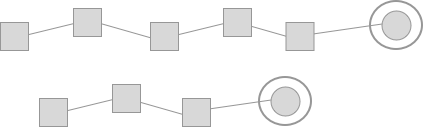
\includegraphics[scale=0.3]{img/exe-feed}
%   \end{center}

\begin{center}
\begin{tabular}{lcl}
$\Delta \ \Lambda^0$         &:& $\times^0$ \\
$\Delta \ \Lambda^{n}$       &:& $\Lambda^{n-1}$ \\
\end{tabular}
\end{center}

   \paragraph{}
   Саме лінійність кінцевого
   процессу виконання певного структурованого або циклічного алгоритму відіграє ключову
   роль у моделюванні віртуальних обчислювальних середовищ. Такі лінеаризовані системи
   уже показали свою ефективність в певному класі обчислень, таких як ланцюгова реплікація,
   реактивні системи, та інші моделі напівгруп навколо певних типів -- протоколів взаємодії між процесами.
   Крім того такі послідовності подій піддаються статистичній обробці для визначення первних кластеризацій
   та інших кореляцій у просторі та часі, тому можна говорити про певні зручні, нормалізовані системи типів для
   такого роду маніпуляцій над даними.

  \subsubsection*{Протоколи повідомлень}

   Простір дій протоколу визначається сумою усіх можливих повідомлень.

\vspace{0.5cm}

\begingroup
\parbox[l][][t]{0.33\textwidth}
{
\begin{tabular}{llll}
$App$       &:& $init$    & $\times\ \_$            \\
            &|& $client$  & $\times\ \_$          \\
            &|& $replay$  & $\times\ \_$          \\
            &|& $\bot$    & \\
\end{tabular}
}
\hspace{0.1cm}
\parbox[l][][t]{0.33\textwidth}
{
\begin{tabular}{llll}
$Store$     &:& $put$     & $\times\ \_$          \\
            &|& $add$     & $\times\ \_$          \\
            &|& $fold$    & $\times\ \_$         \\
            &|& $\bot$    & \\
\end{tabular}
}
\hspace{0.1cm}
\parbox[t][][t]{0.33\textwidth}
{
\begin{tabular}{llll}
$Proc$      &:& $spawn$       & $\times\ \_$      \\
            &|& $complete$    & $\times\ \_$         \\
            &|& $run$         & $\times\ \_$          \\
            &|& $\bot$        &
\end{tabular}
}
\endgroup

\newpage
  \subsubsection*{Лямбда числення}

Для розробки нашої теорії ми застосуємо інтуітіоністську теорію типів Мартіна Льофа.
Ця система типів буде застосовуватися для довення робочих теорем. База мови складає
лябмда числення як внутрішня мова декартово-замкненої категорії. Лямбда числення в своїй
основі скаладається з конструктора типу яка визначає функції та елімінатора -- аплікації
функції до аргументу.

\begingroup
\parbox[t][][l]{0.40\textwidth}{

\begin{prooftree}
\AxiomC{$\Gamma\ x:A \vdash\ B$ }
\UnaryInfC{$\Gamma \vdash fun\ x : A \rightarrow B$}
\end{prooftree}

}
\hspace{0.1cm}
\parbox[t][][r]{0.60\textwidth}{

\begin{prooftree}
\AxiomC{$\Gamma\ f:A \rightarrow B$ }
\AxiomC{$\Gamma\ a:A$ }
\BinaryInfC{$\Gamma \vdash f \ a : B$}
\end{prooftree}

}
\endgroup

  \subsubsection*{Алегбраїчні типи даних}

Далі йде внутрішня мова алгебраїчних типів даних яка складається з суми та добутку,
за допомогою яких контруюються суми-протоколи та кортежі-пакети, а також {\bf nil} типу-атому,
яким зручно термінувати рекурсивні типи даних, такі як {\bf cons}.

\begin{prooftree}
\AxiomC{}
\UnaryInfC{$\Gamma \vdash\ \bot$ }
\end{prooftree}

\begingroup
\parbox[t][][l]{0.40\textwidth}{

\begin{prooftree}
\AxiomC{$\Gamma \vdash\  a:A$ }
\AxiomC{$\Gamma \vdash\  b:B$ }
\BinaryInfC{$\Gamma \vdash\  (a,b) : A \times B$ }
\end{prooftree}

\begin{prooftree}
\AxiomC{$\Gamma \vdash\  a:A$ }
\AxiomC{$\Gamma \vdash\  b:B$ }
\BinaryInfC{$\Gamma\vdash a\ |\ b : A \otimes B$}
\end{prooftree}

}
\hspace{0.1cm}
\parbox[t][][r]{0.60\textwidth}{


\begin{prooftree}
\AxiomC{$\Gamma\ x: A \times B$ }
\UnaryInfC{$\Gamma \vdash fst\ x : A$;
           $\Gamma \vdash snd\ x : B$}
\end{prooftree}

\begin{prooftree}
\AxiomC{$\Gamma\ x: A \otimes B$ }
\UnaryInfC{$\Gamma \vdash inl\ x : A$;
           $\Gamma \vdash inr\ x : B$}
\end{prooftree}


}
\endgroup


  \subsubsection*{Процеси і протоколи}

Також ми анонсуємо процес як фундаменльний тип даних, подібний до функції але який здатний
тритати певний стан у вигляді типа коротежа та бути здатним реагувати на повідомлення суми.

\begin{prooftree}
\AxiomC{$\Gamma\ \vdash e : Error$ }
\AxiomC{$\Gamma\ \vdash h : History$ }
\BinaryInfC{$\Gamma \vdash module : a : \Sigma \times P \rightarrow P $}
\AxiomC{$\Gamma\ \vdash env : Document$ }
\AxiomC{ $\Gamma\ \vdash s : Event | Task | Flow$ }
\TrinaryInfC{$\Gamma \vdash p : Process$}
\end{prooftree}

\begin{prooftree}
\AxiomC{$\Gamma\ \vdash \Sigma, X$ }
\AxiomC{$\Gamma\ \vdash p : Process$ }
\BinaryInfC{$\Gamma \vdash {spawn}_{\Sigma}\ p : \pi $}
\end{prooftree}

\begin{prooftree}
\AxiomC{$\Gamma\ \vdash spawn : \pi$ }
\AxiomC{$\Gamma\ \vdash m : \Sigma$ }
\BinaryInfC{$\Gamma \vdash {join}_{\Sigma}\ (m, spawn) \rightarrow \Sigma$;
            $\Gamma \vdash {async}_{\Sigma}\ (m, spawn) \rightarrow \Sigma$}
\end{prooftree}


\newpage

  \subsubsection*{Логіка та квантори}

Далі йдуть квантори $\forall$ та $\exists$ які теж виражаються як конструкції типів:

\begingroup
\parbox[t][][l]{0.40\textwidth}{

\begin{prooftree}
\AxiomC{$\Gamma\ x: A \vdash B$ }
\AxiomC{$\Gamma\ \vdash A$ }
\BinaryInfC{$\Gamma\ \vdash \Pi (x : A) B $}
\end{prooftree}

\begin{prooftree}
\AxiomC{$\Gamma\ x: A \vdash B$ }
\AxiomC{$\Gamma\ \vdash A$ }
\BinaryInfC{$\Gamma\ \vdash \Sigma (x : A) B $}
\end{prooftree}

}
\hspace{0.1cm}
\parbox[t][][r]{0.60\textwidth}{

\begin{prooftree}
\AxiomC{$\Gamma\ \vdash a : A$ }
\AxiomC{$\Gamma\ x : A \vdash B$ }
\AxiomC{$\Gamma\ b : B (x=a)$ }
\TrinaryInfC{$\Gamma\ \vdash (a,b) : \Pi (x : A) B $}
\end{prooftree}


\begin{prooftree}
\AxiomC{$\Gamma\ \vdash a : A$ }
\AxiomC{$\Gamma\ x : A \vdash B$ }
\AxiomC{$\Gamma\ b : B (x=a)$ }
\TrinaryInfC{$\Gamma\ \vdash (a,b) : \Sigma (x : A) B $}
\end{prooftree}

}
\endgroup

\begingroup
\parbox[t][][l]{0.40\textwidth}{

\begin{prooftree}
\AxiomC{$\Gamma\ \vdash x: A$ }
\AxiomC{$\Gamma\ \vdash x': A$ }
\BinaryInfC{$\Gamma\ \vdash Id_A (x,x')$}
\end{prooftree}

}
\hspace{0.1cm}
\parbox[t][][r]{0.60\textwidth}{

}\endgroup


\begin{center}
\begin{tabular}{lll}
  рефлексивність &:& $Id_A(a,a)$ \\
  підстановка     &:& $Id_A(a,a') \rightarrow B(x=a) \rightarrow B(x=a')$ \\
  симетричність  &:& $Id_A(a,b) \rightarrow Id_A(b,a)$  \\
  транзитивність &:& $Id_A(a,b) \rightarrow Id_A(b,c) \rightarrow Id_A(a,c)$ \\
  конгруентність &:& $(f: A \rightarrow B) \rightarrow Id_A(x,x') \rightarrow Id_B(f(x),f(x'))$ \\
\end{tabular}
\end{center}



  \subsubsection*{Контраваріантні процеси}

  Ко-процеси це моноїди з перевернутою стрілкою, які визначають зворотній шлях виконання
  події та обернену зміни стану в зворотньому порядку. З точки зоро типів нічого не змінюється,
  однак оберненої функції-фунтора процесу-моноїда може і не існувати. Процеси які є
  одночасно коваріантними та контраваріантними називаються інваріантними процесами, сигнатура яких
  алгебраїчно збігається з сигнатурою бінарного дерева.

\begin{center}
\begin{tabular}{lcl}
$X$         &:& $\times^{i}$ \\
$\Lambda$   &:& $\times^{4} \ I \ X \ \Lambda_{next} \ \Lambda_{prev}$ \\
            &|& $\bot$ \\
\end{tabular}
\end{center}

\begin{center}
$st(p) = p(st-1)$ — застосування функції до протокольної заявки та стану процесу
$p-1(st) = st-1$ — обернена функція
\end{center}

  \subsubsection*{Типи процесів}

\begin{center}
\begin{tabular}{lll}
         $action$ &:& ${proc}_{Proc}\ (Proc\ |\ \Sigma) \times process \rightarrow process$ \\
         $event$  &:& ${proc}_{App}\ (App\ |\ \Sigma) \times cx \rightarrow cx$ \\
         $operation$    &:& ${proc}_{Store}\ (Store\ |\ \Sigma) \times container \rightarrow container$ \\
\end{tabular}
\end{center}

\newpage

\subsection*{Віртуальна машина}

\begin{figure}[h!]
\centering
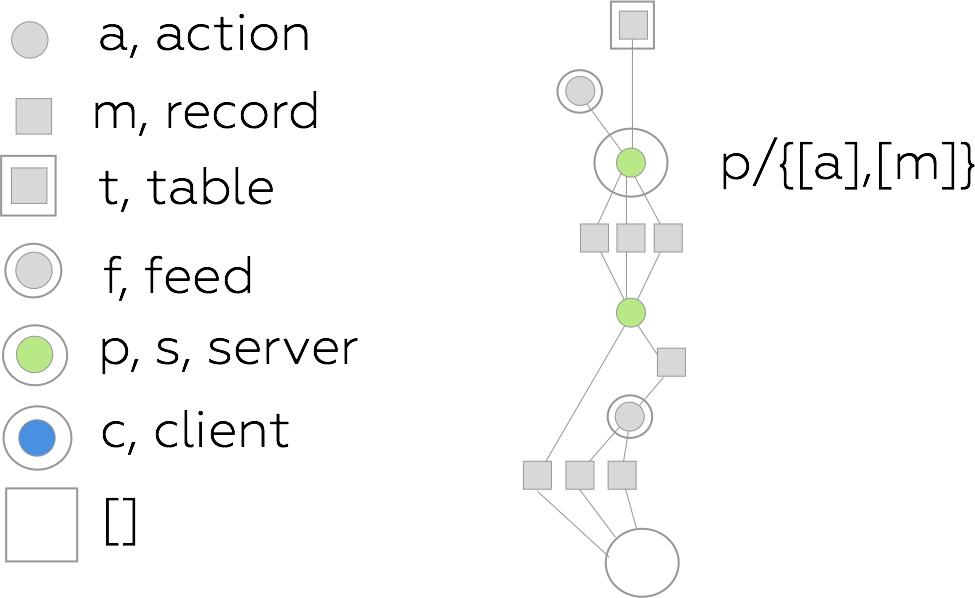
\includegraphics[scale=0.3]{img/exe-legend}
\caption{Базові елементи віртуального середовища}
\end{figure}

{\bf action} is the piece of code applied to message using pattern matching.\\
{\bf record} is the tuple that defines a protocol.\\
{\bf client} is the true customer of the system who is using service on daily basis.\\
{\bf server} is the process nicely scheduled by the system.\\
{\bf feed} is the server managed list of records.\\
{\bf table} is the ixset or ets based queryable tables.\\

\subsection*{Сигнатури сервісів}

{\bf app} is the web clients monoidal state machine.\\
{\bf proc} is the oriented graph monoidal executional engine.\\
{\bf store} is the 2-category key-value database.\\

\begin{center}
\begin{tabular}{lll}
           $store^3$ &:& $\times^3 \Lambda_{id_seq}\ \Lambda_{table}\ \Lambda_{feed}$ \\
          $roster^2$ &:& $\times^2 \Lambda_{feed}\ \Lambda^2_{feed}$ \\
             $app^2$ &:& $\times^2 \Lambda_{session}\ \Lambda_{proc}$ \\
           $depot^1$ &:& $\times^1 \Lambda_{account}$ \\
             $act^1$ &:& $\times^1 \Lambda_{proc}$ \\
\end{tabular}
\end{center}

\newpage
\subsection{Персистентність послідовностей}

Для забезпечення персистентного зберігання послідовностей використовується
очевидний спосіб зберігання елементів послідовності у key-value сховищі разом
з референсами на наступні, та у випадку контраварінтних процесів, також і на
попередні елементи у послідовності. Таким чином ми можемо перелічити усі
елементи послідовності. Акумулятор розділеної у просторі та часі операції
накопичує усі необхідні агрегації після кожної операції з послідовністю. Таким
чином похідна від алгебраїчної структури списку буде скаляр-акумулятор після
завершення перелічення.

\begin{figure}[h!]
\centering
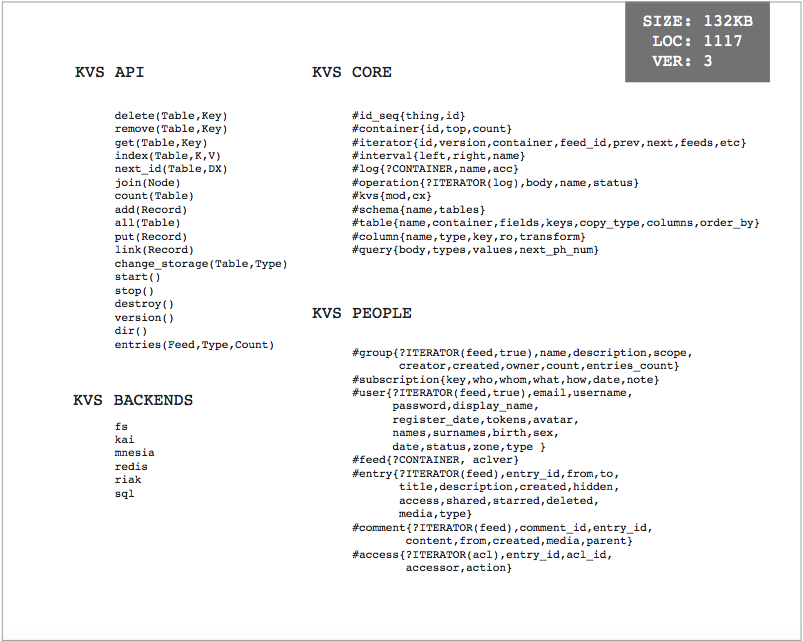
\includegraphics[scale=0.4]{img/exe-kvs-api}
\caption{Типи, функції та модулі}
\end{figure}

В даній роботі ми розглянемо формальні визначення сховища, його референсів, послідовностей через рекурсивні
алгебраїчні типи даних та процеси, черги яких забезпечують впорядкованість послідовності
запитів до послідовностей, що веде до лінійності операції у часі.

\begin{figure}[h!]
\centering
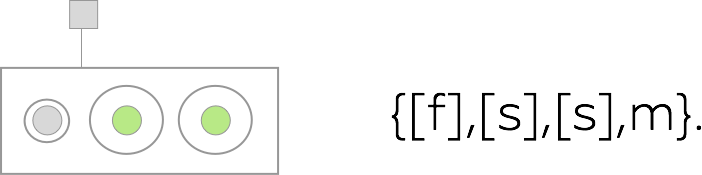
\includegraphics[scale=0.4]{img/exe-kvs}
\caption{Послідовності ключів, таблиць, індексів та інтерфейс}
\end{figure}

\newpage
\subsection{Мультипротокольный чат}

\begin{figure}[h!]
\centering
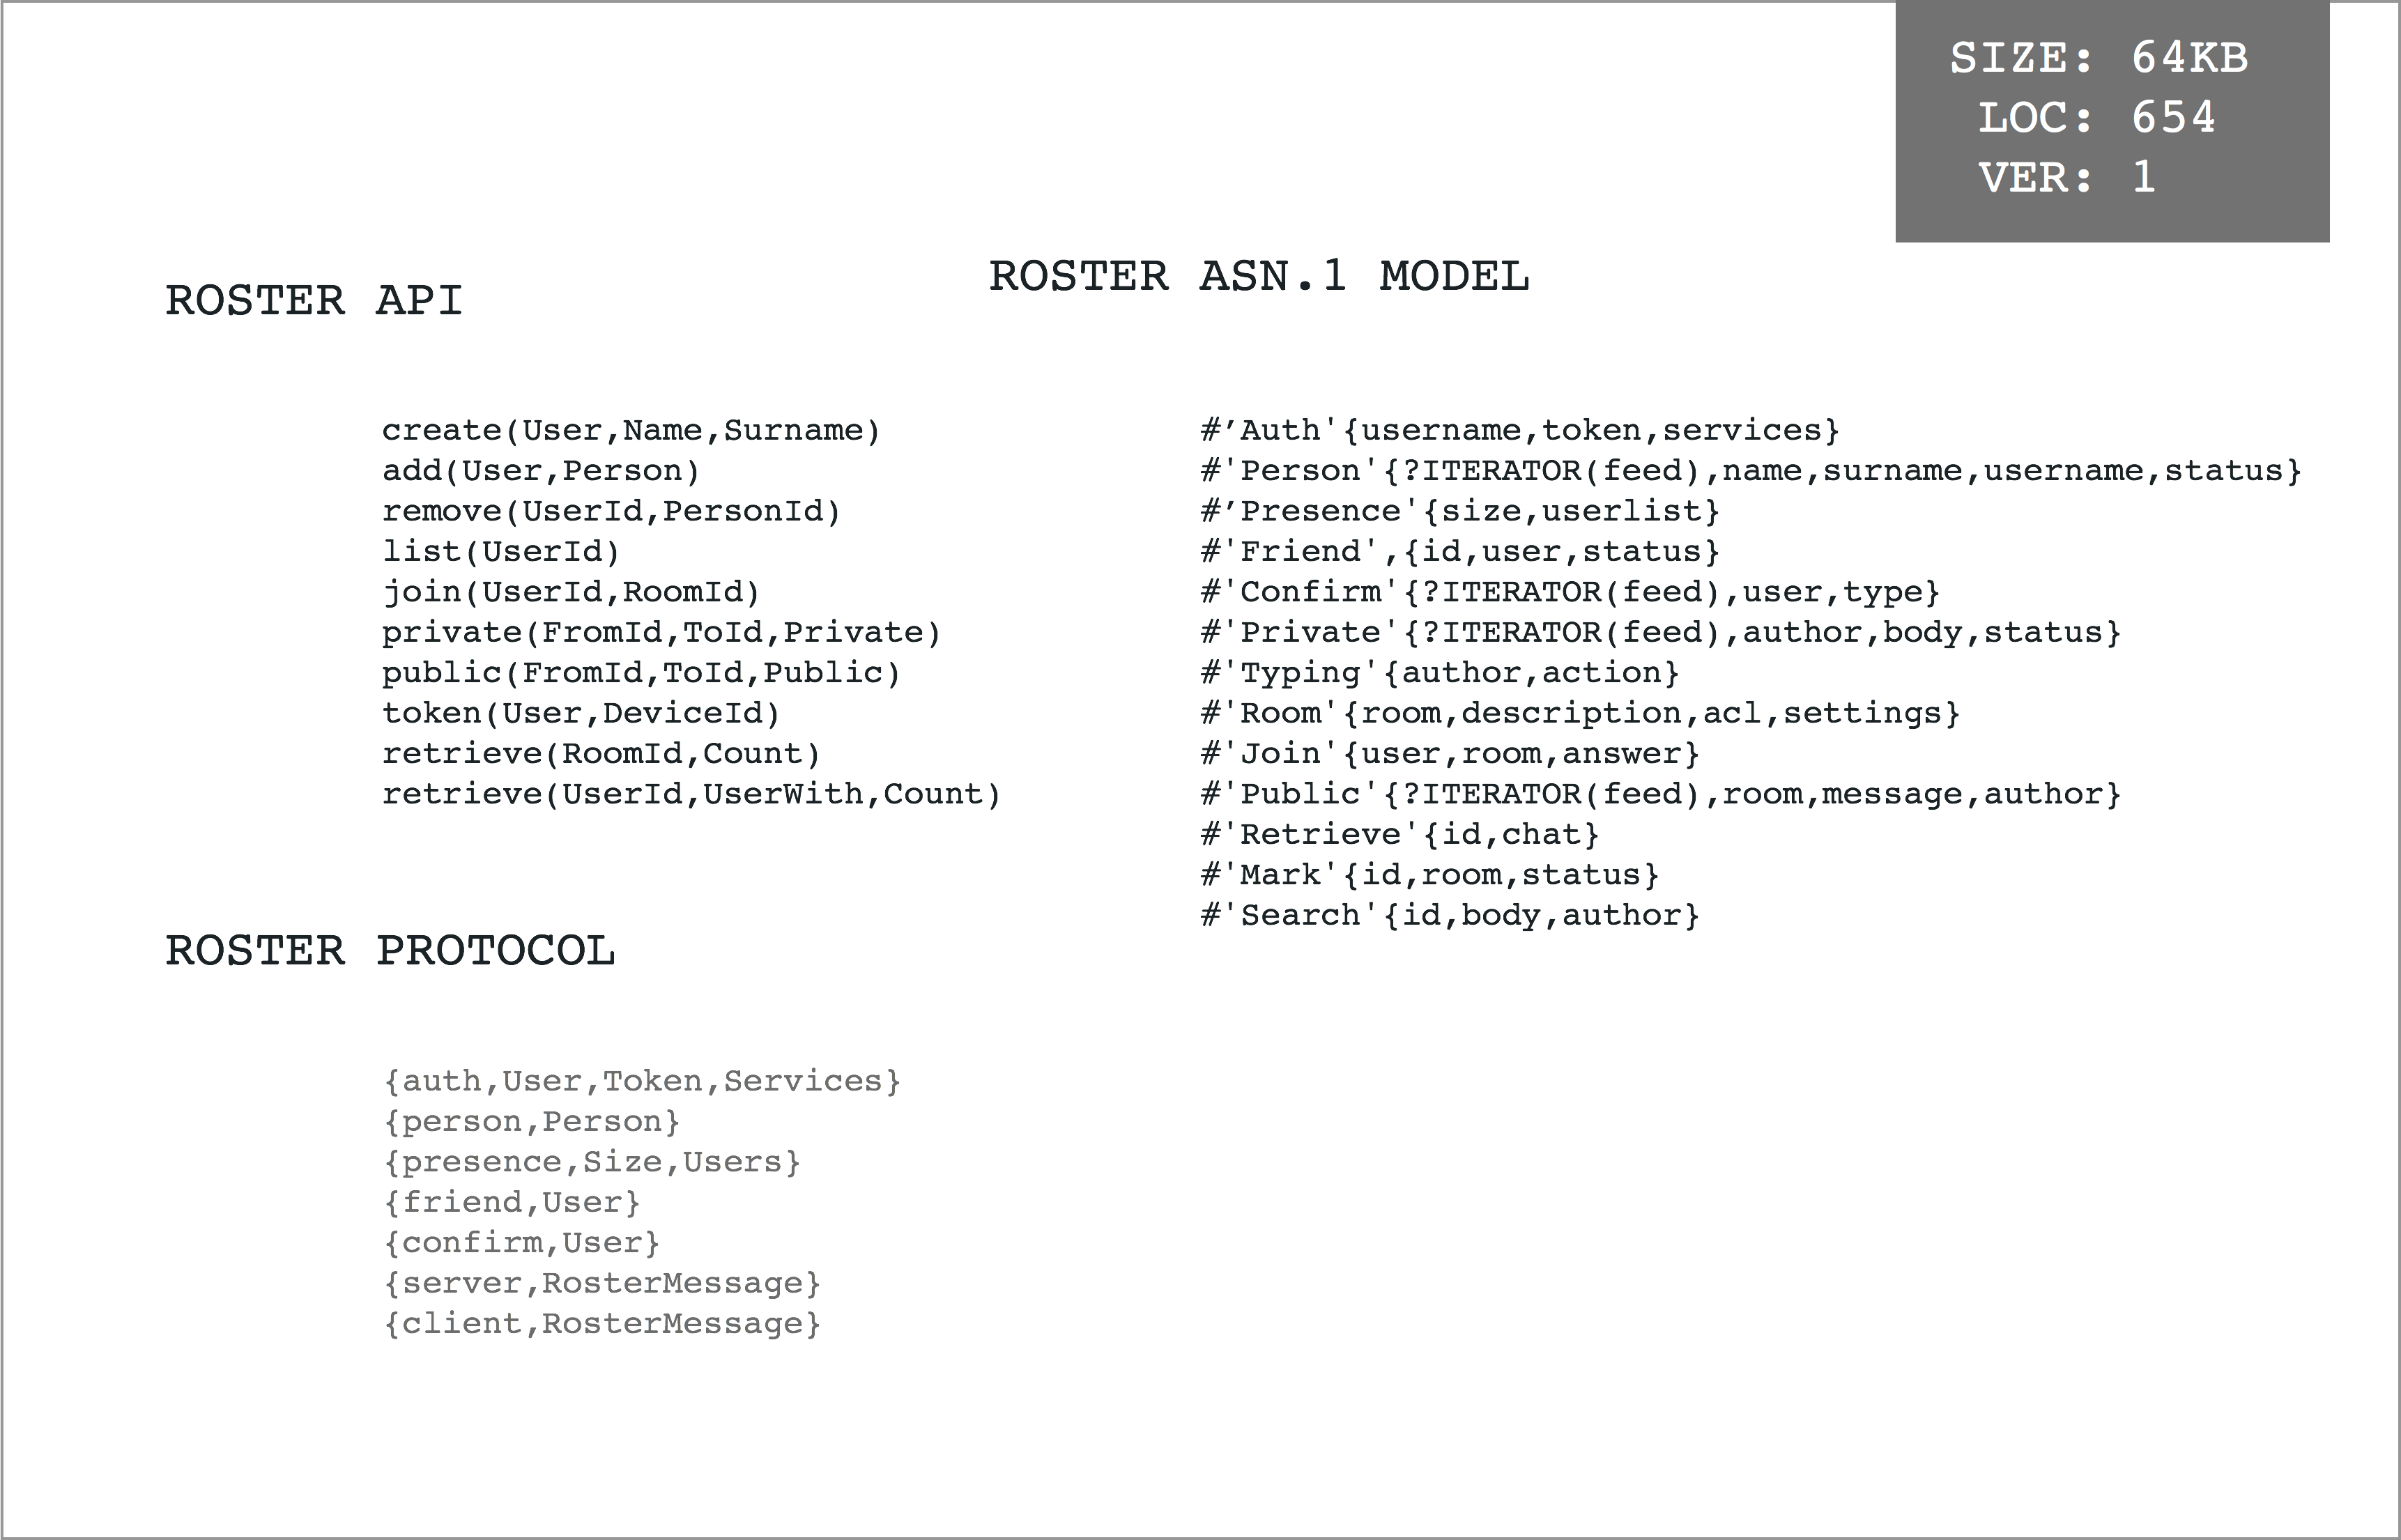
\includegraphics[scale=0.1]{img/exe-roster-api}
\caption{Типи, функції та протокол}
\end{figure}

\begin{figure}[h!]
\centering
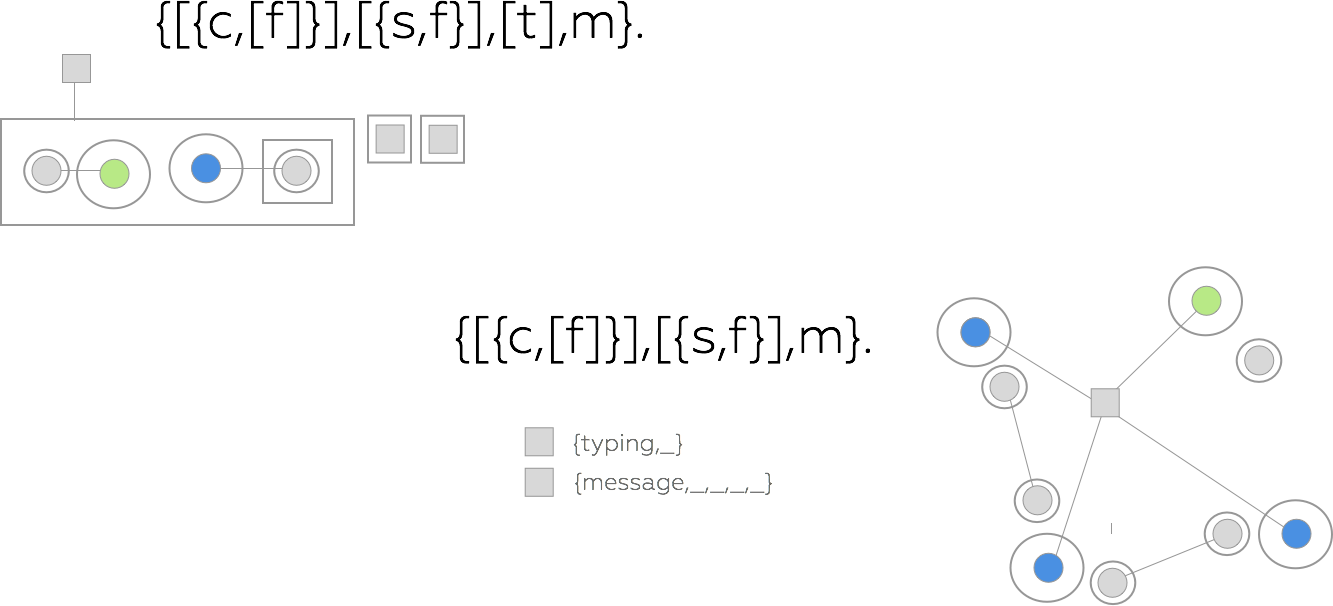
\includegraphics[scale=0.3]{img/exe-roster}
\caption{Cписки кімнат та користувачів і їхні чати, дві таблиці та протокол}
\end{figure}


\newpage

%\newpage
\subsection{Мета дослідження}
\vspace{0.5cm}
   Основною метою дослідження є збезпечення виконання критеріїв відповідності
   показників ефективності, детермінованості та якості шляхом впровадження
   результату даної теорії, комплексу програмного забезпечення у виробничий процес.

   За рахунок компактності передбачається значна економія складності та простота у експлуатації,
   що веде до сниження собівартості впровадження. Коректність передбачає заміну
   автоматозаваному тестуванню, а закритість середовища дозволяє гнучко використовувати
   середовище на різних виробничих платформах.
   \\

\subsection{Результати}
\vspace{0.5cm}
   Одна з останніх систем, яка була впроваджена для заміни існуючої системи, мала
   показники у співвідношенні розміру 10, швидкості 20 та виконання 3. Інші системи
   у історичній послідовності мали ці показники такими 10, 2, 8, та 19, 5, 5.
   В середньому показники ефективності відрізняються більше ніж на пів порядка
   в кращу сторону після впровадження продуктів на базі розробленої моделі.
   Існують продукти також і на інших мовах програмування.

\newpage
\begin{thebibliography}{9}

\bibitem{lof}      Per Martin-Löf \textit{Intuitionistic Type Theory.} 1984
\bibitem{erl}      J.Armstrong. \textit{Making reliable distributed systems in the presence of sodware errors.} 2003.
\bibitem{comm}     Robin Milner. \textit{ A Calculus of Communicating Systems.} 1986.
\bibitem{lawvere}  William Lawvere. \textit{Conceptual Mathematics.} 1997.
\bibitem{pierce}   Benjamin Pierce. \textit{Basic category theory for computer scientist.} 2004.
\bibitem{mclane}   Сандерс Мак Лейн. \textit{Категории для работающего математика.} 2004.
\bibitem{tla}      Leslie Lamport. \textit{Specifying Systems.} 2004.
\bibitem{barrtri}  Michael Barr and Charles Wells. \textit{Toposes, Triples and Theories.} 2000.
\bibitem{barrcat}  Michael Barr and Charles Wells. \textit{Category Theory for Computing Science.} 1995.
\bibitem{bakur}    И.Бакур, А.Деляну. \textit{Введение в теорию категори и функторов.} 1972.
\bibitem{commpi}   Robin Milner. \textit{Communicating and Mobile Systems: The $\pi$-calculus.} 1999.
\bibitem{polypi}   Robin Milner. \textit{The Polyadic $\pi$-Calculus: A Tutorial.} 1993.
\bibitem{mass}     Коваленко. \textit{Теория Массового Обслуживания.} 1965.
\bibitem{meseguer} Meseguer, Montanari.  \textit{Petri Nets Are Monoids.} 1990.
\bibitem{waddual}  Philip Wadler \textit{Call-by-Value is Dual to Call-by-Name.} 1000
\bibitem{seserl}   D.Mostrous, V.Vasconcelos \textit{Session Typing for a Featherweight Erlang.} 1990.
\bibitem{suberl}   S.Marlow, P.Wadler \textit{A practical subtyping system for Erlang.} 1997
\bibitem{upserl}   A.Lindgren \textit{A Prototype of a Soft Type System for Erlang.} 1996
\bibitem{mcbride}  C. McBride. \textit{Dependently Typed Func- tional Programs and their Proofs.} 1999
\bibitem{mcbrider} C. McBride. \textit{The Derivative of a Regular Type is its Type of One-Hole Contexts.}
\bibitem{schwarz}  C. Schwarzweller. \textit{Mizar Veri cation of Generic Algebraic Algorithms.} 1997
\bibitem{mourael}  L.Moura., S.Kong \textit{Elaboration in Dependent Type Theory.} 1997
\bibitem{coqhuet}  T.Coquand, G.Huet \textit{The Calculus of Constructions.} 1988
\bibitem{lampax}   L.Lamport \textit{Paxos Made Simple.} 2001
\bibitem{chipvm}   A.Chlipala \textit{Certified Programming with Dependent Types} 2015
\end{thebibliography}

\end{document}
